\chapter{Introducción}

\section{Motivación}
Para motivar el tema a tratar en este trabajo, presentamos el siguiente problema que
perfectamente se podría presentar en un escenario real.\\
El tribunal de la libre competencia (TDLC) desea desarrollar una plataforma que permita
a las distintas empresas presentar pruebas que inculpen
a otra empresa en delitos como colusión, monopolio, etc. Para ello ha puesto
a disposición de las empresas un conjunto de servidores a los cuales enviar sus denuncias.\\
Para no amedrentar a una empresa
denunciante  es necesario que la comunicación entre la empresa y cada servidor
sea anónima. Pues de este modo ningún observador podría determinar que una empresa a denunciado
a otra de cierto delito y tomar represalias.\\
Por otro lado el TDLC confía más en el testimonio de algunas empresas que en el de otras, ya sea por
su conducta anterior u otros factores. Por lo tanto desea estar completamente seguro de la identidad
de una empresa cuando esta empresa presente pruebas usando la plataforma, pues así puede determinar
un factor de credibilidad en la denuncia.\\
La plataforma se diseña para operar en internet, por lo tanto debe mantener sus propiedades
de seguridad inclusive si es ejecutada concurrentemente con protocolos maliciosos.\\
Para desarrollar la plataforma, el TDLC ha determinado que su problema es exactamente el siguiente:\\
\textit{Desea crear un protocolo mediante el cual las empresas se comuniquen con cada uno de los servidores
de denuncias. La comunicación entre empresas y servidores debe ser anónima y autentificada, y esto se
debe cumplir inclusive si el protocolo es ejecutado concurrentemente con otros protocolos.}\\ 

\section{Descripción del problema}

En general, el problema anterior puede aplicarse a cualquier de grupo de personas que
desean comunicarse entre sí en una red (internet o una red local) y desea obtener garantías
similares. A continuación iniciamos el camino de formalización del problema motivacional.\\
La solución del problema consiste en encontrar un protocolo (un algoritmo distribuido) de cual
se puedan garantizar matemáticamente las siguientes tres propiedades :
\begin{enumerate}
    \item Anonimato
    \item Autentificación desmentible
    \item Componibilidad
\end{enumerate}

\subsubsection{Anonimato}
A modo de ejemplo podemos considerar un protocolo ``usual" de comunicación, un protocolo IP simplificado.
En la Figura \ref{tcpip_simple} cada flecha de $A$ a $B$ indica que $A$ envió un mensaje a
$B$. La etiqueta de una flecha de $A$ a $B$ indica el mensaje intercambiado en la ejecución de protocolo.
Por ejemplo Empr-1 envió a Serv-1 el mensaje $(m_{e1s1}, ip_{e1}, ip_{s1})$, donde $m_{e1s1}$ es el contenido
del mensaje, $ip_{e1}$ es la dirección IP de la Empresa 1 e $ip_{s1}$ es la dirección IP del Servidor 1.
Notemos que estos
datos son necesarios para poder \textit{rutear} los mensajes de un participante a otro, pero a la vez 
se revela a un observador que Empr-1 envió un mensaje a Serv-1. Por lo tanto podemos decir que
\textbf{el protocolo IP simplificado no es anónimo} pues \textbf{existe un ataque}.\\

\begin{figure}[hp]
    \centering
    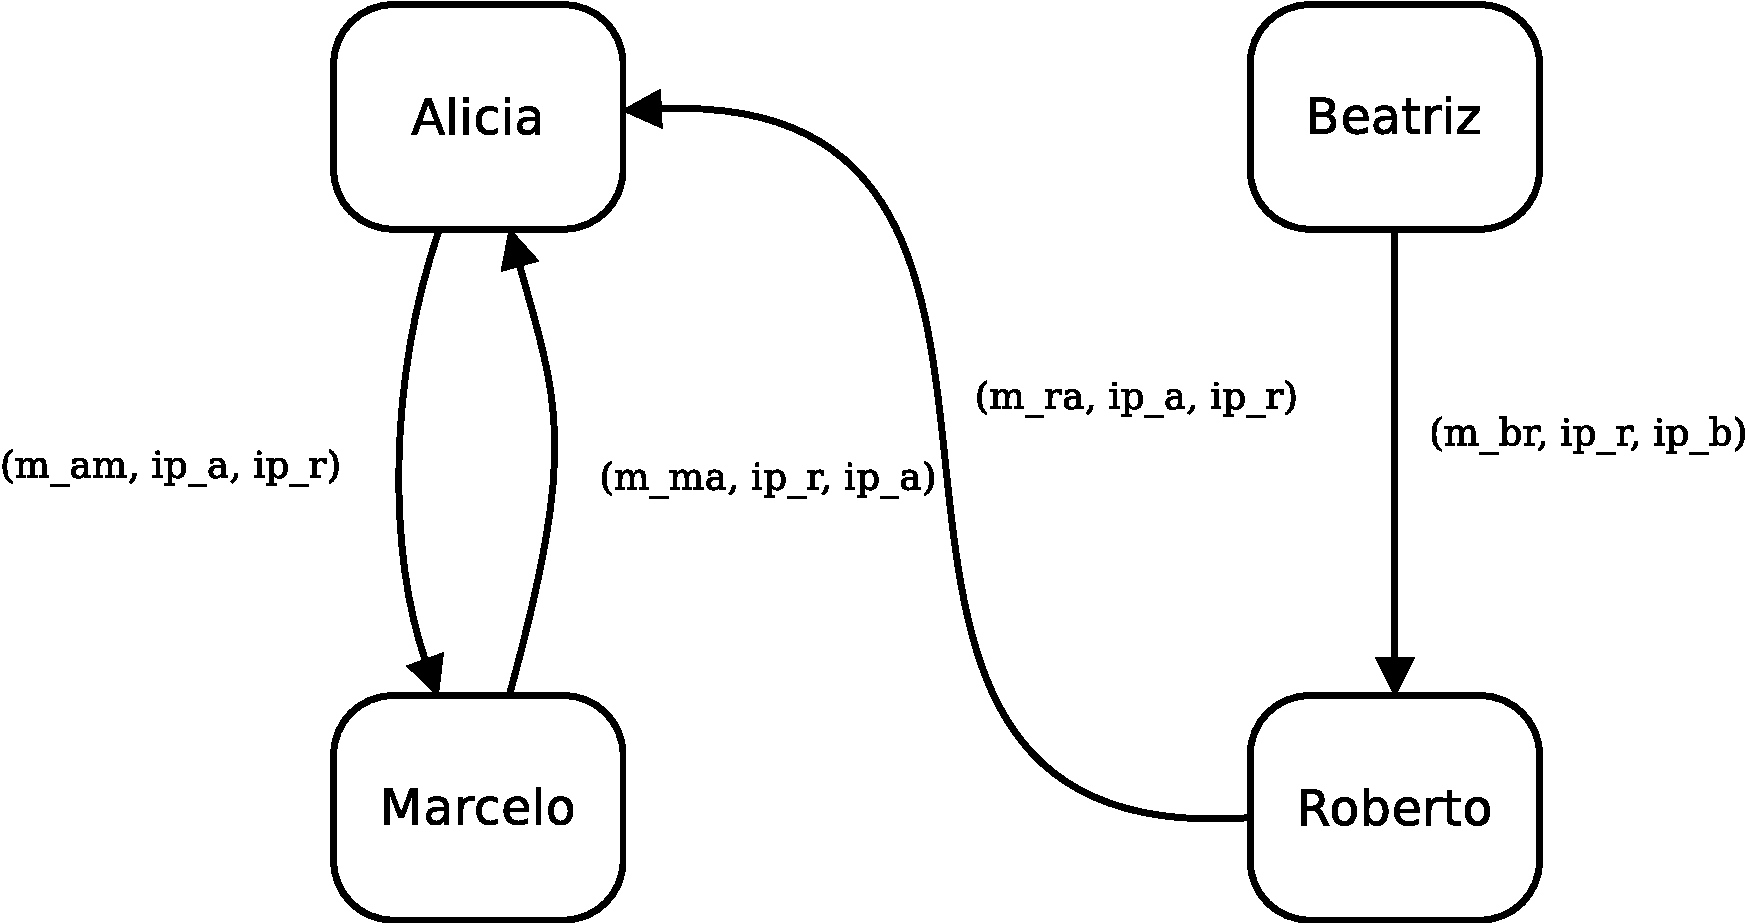
\includegraphics[width=0.7\textwidth]{figs/tcpip_simple}
    \caption{Protocolo simple de comunicación}
    \label{tcpip_simple}
\end{figure}

Para definir el anonimato resulta crucial definir formalmente que es considerado
un ataque al anonimato, pues un protocolo es anónimo si y solo si no existe ningún ataque.
En \cite{conf/pet/HeviaM08} se define un ataque con el siguiente juego.
El observador o adversario determinada dos posibles ejecuciones del protocolo, las cuales difieren en
qué mensajes son enviados por quién y qué mensajes son recibidos por quién. Entonces
consideraremos que el adversario realiza un ataque si al ejecutar al adversario con cada una
de las posibles ejecuciones del protocolo, el adversario logra identificar cuál es cuál.
Por lo tanto un protocolo sera seguro si y solo si cualquier adversario no logra distinguir
una ejecución de otra.

\subsubsection{Autentificación desmentible}
En el protocolo de la Figura \ref{tcpip_simple} es posible que un adversario (rol que puede
asumir una empresa $Empr-2$) se haga pasar por una empresa $Empr-1$ con buena reputación y denuncie
falsamente a una empresa enemiga $Empr-3$. Para ello
sólo es necesario que modifique uno de sus mensajes cambiando $ip_e2$ por $ip_e1$.
Por lo tanto decimos que el protocolo no implementa canales autentificados.\\
Con canales autentificados nos referimos protocolos en los cuales es posible estar seguro,
con alta probabilidad, de quién es el autor de un mensaje. Sin embargo hay que ser cuidadoso
con el protocolo de autentificación usado, pues los más conocidos
(firmas digitales por ejemplo) poseen la propiedad de \textit{non repudiability}. Esto es,
que el emisor de un mensaje autentificado no puede negar a ``la comunidad" que él es el autor
del mensaje. Esto estaría contradiciendo el anonimato, pues el adversario también sería capaz
de asociar la autoría de un mensaje a el emisor de éste.\\
La autentificación desmentible, introducida en \cite{DwoNaoSah04}, se refiere a los protocolos
que implementan canales anónimos con la propiedad adicional de que cada mensaje es autentificado
a un receptor específico y el receptor no es capaz de probar a nadie más quién es el autor del mensaje.

\subsubsection{Componibilidad}
En general, el hecho de implementar protocolos con ciertas garantías (por ejemplo ano\-ni\-ma\-to y
autentificación desmentible) no garantiza que dichas propiedades se sigan teniendo cuando
el protocolo es ejecutado concurrentemente con otros protocolos.\\
En \cite{conf/focs/Canetti01}, Canetti introduce el \textit{framework} criptográfico conocido
como \textit{Universal Composabillity} (desde ahora UC). UC propone una metodología para definir y
demostrar los objetivos de seguridad de un protocolo (por ejemplo anonimato y autentificación)
de un protocolo. UC garantiza que el protocolo mantiene su seguridad inclusive
si es ejecutado concurrentemente con cualquier protocolo, siempre y cuando no comparta estado
con el protocolo analizado.\\
Cuando el protocolo sí comparte estado con otros protocolo es necesario hacer uso del
\textit{framework Generalized Universal Composabillity} (desde ahora GUC), que generaliza a UC.
Informalmente GUC propone una metodología para incluir el estado que un protocolo podría compartir
con otros.

\section{Objetivos}

\subsection{Objetivo general}
Diseñar un protocolo criptográfico eficiente que cumpla nociones razonables
de Anonimato y Autentificación Desmentible. Demostrar matemáticamente su
seguridad usando herramientas modernas de análisis criptográficas (GUC) y
estudiar su relación con otras primitivas criptográficas.

\subsection{Objetivos específicos}

\begin{enumerate}
    \item Estudiar conceptos asociados a interacciones desmentibles y las técnicas y
          primitivas criptográficas asociadas (encriptación y mecanismos de autentificación
           como firmas digitales y esquemas de identificación).
    \item Estudiar conceptos de anonimato y las técnicas y primitivas criptográficas
          asociadas.
    \item Proponer un protocolo que combine ambas nociones.
    \item Analizar dicho protocolo en términos de efectividad y eficiencia.
    \item Analizar la efectividad en términos de las garantías de seguridad obtenidas.
    \item Analizar la eficiencia en términos de los costos en tiempo asociados al
          protocolo.
    \item Estudiar su relación con otros protocolos criptográficos.
\end{enumerate}


En la Figura \ref{sigmix_simple} se muestra un diagrama para explicar nuestra solución. A grandes
razgos, proponemos combinar un protocolo de autentificación desmentible con un protocolo de
canales anónimos. Es por ello que primero los mensajes enviados son procesados por el protcolo de
autentificación desmentible para luego ser distribuidos por el protocolo de canales anónimos.

\begin{figure}[hp]
    \centering
    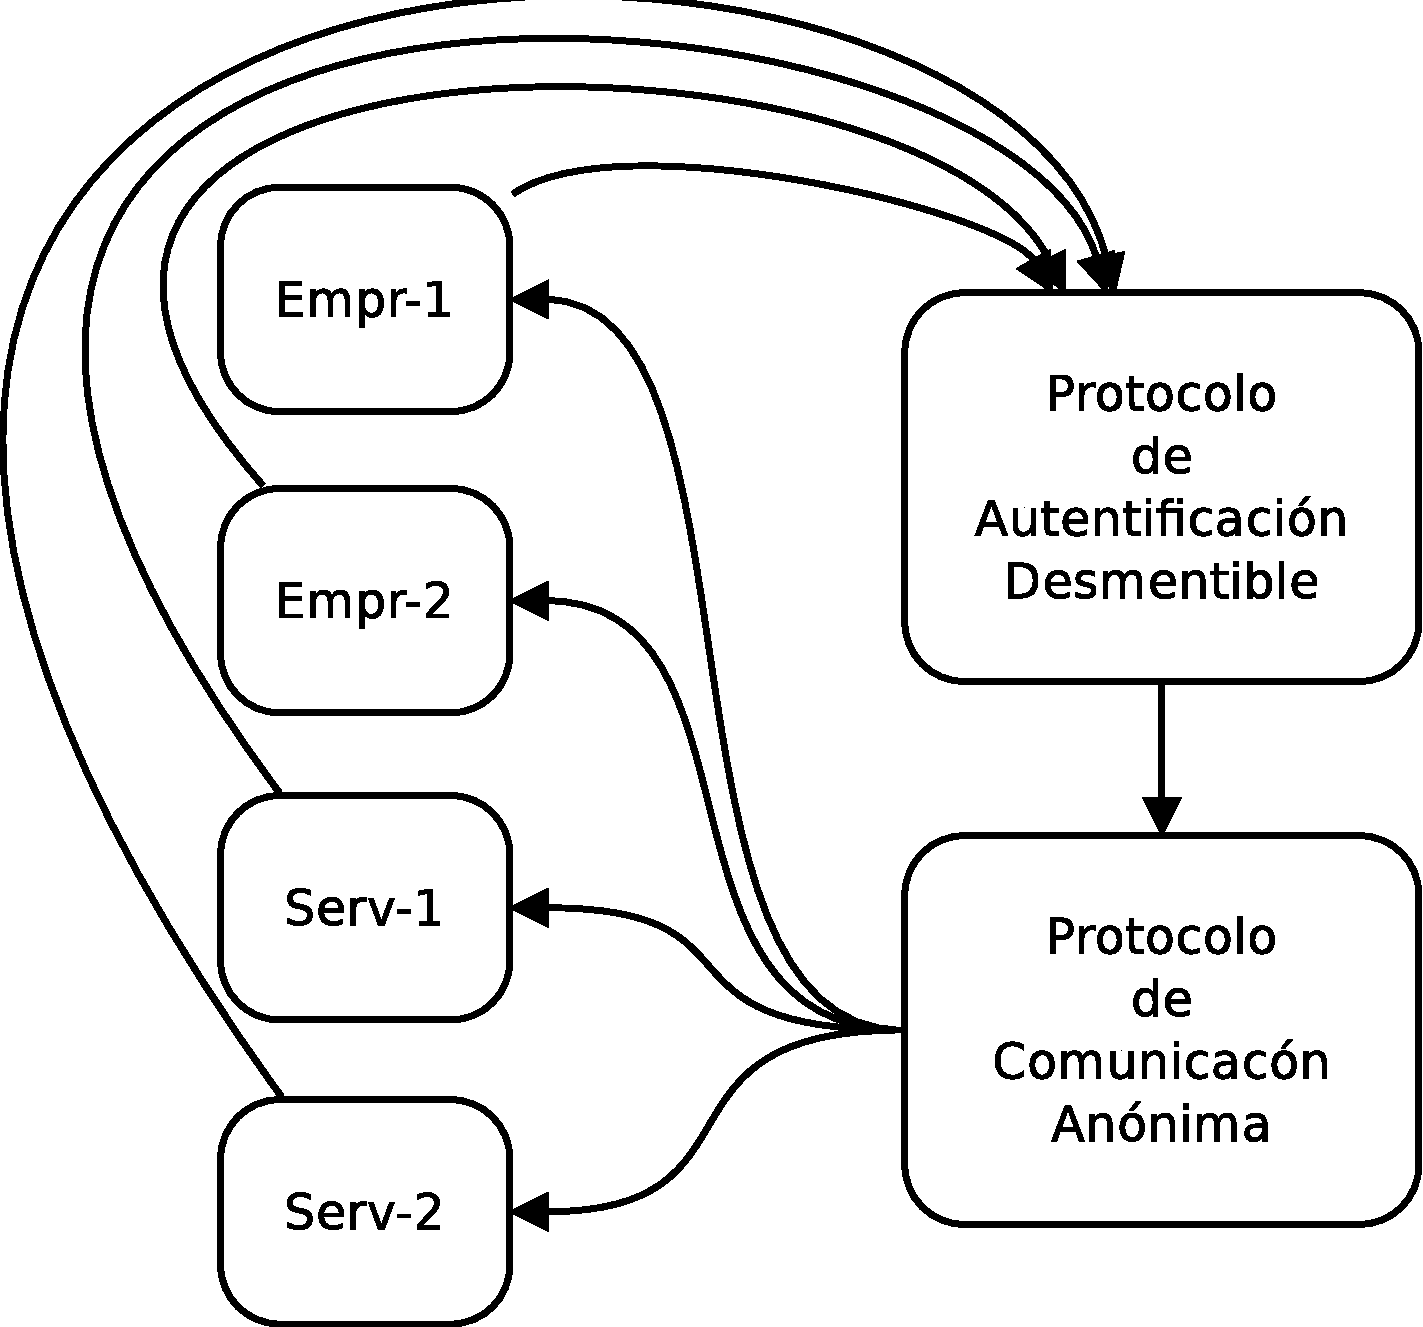
\includegraphics[width=0.5\textwidth]{figs/sigmix_simple}
    \caption{Solución propuesta}
    \label{sigmix_simple}
\end{figure}

